% =============================================================================
% main.tex -- Reviews in Fish Biology and Fisheries submission
% Compile: latexmk -pdf main.tex
% Structure: 1 Introduction | 2 Literature synthesis (methods + findings)
%            3 Simulation study (design + results) | 4 Roadmap | 5 Discussion
% Springer's sn-jnl class can replace the preamble at submission.
% =============================================================================
\documentclass[12pt,a4paper]{article}
\usepackage[margin=25mm]{geometry}
\usepackage[utf8]{inputenc}
\usepackage[T1]{fontenc}
% \usepackage{lmodern}  % uncomment if the lmodern package is installed
\usepackage{amsmath,amssymb}
\usepackage{graphicx}
\usepackage{booktabs}
\usepackage{array}
\usepackage{longtable}
\usepackage{float}
\usepackage{caption}
\usepackage{setspace}
\usepackage{lineno}
\usepackage[authoryear,round,sort]{natbib}
\usepackage[hidelinks]{hyperref}
\usepackage{xcolor}
\graphicspath{{figures/}}
% panel helper: letter set in the document, not inside the image
\newcommand{\panel}[3]{\begin{minipage}[t]{#2}\raggedright\textbf{(#1)}\\[2pt]\includegraphics[width=\linewidth]{#3}\end{minipage}}

\captionsetup{labelfont=bf,labelsep=space,font=small}
\renewcommand{\figurename}{Fig.}
\bibliographystyle{plainnat}  % submit with spbasic (Springer); plainnat used for local build
\setcitestyle{aysep={}}
\doublespacing
\linenumbers

% Numbers and generated tables come from the R scripts; nothing is typed by hand.
% results.tex -- GENERATED by scripts/make_results_macros.R. Do not edit.
% generated 2026-10-23 12:05:35.890232
\newcommand{\nScenarios}{108}
\newcommand{\nPanels}{120}
\newcommand{\nReplicates}{10}
\newcommand{\nDatasets}{1080}
\newcommand{\nFits}{5526}
\newcommand{\nFitsMain}{5400}
\newcommand{\waMax}{6.51}
\newcommand{\waCum}{192.7}
\newcommand{\waDur}{60}
\newcommand{\naiveBiasLagZero}{-0.016}
\newcommand{\naiveBiasLagOne}{0.065}
\newcommand{\naiveBiasLagTwo}{0.069}
\newcommand{\lagoneBiasLagZero}{0.058}
\newcommand{\lagoneBiasLagOne}{-0.016}
\newcommand{\lagoneBiasLagTwo}{0.065}
\newcommand{\dlnmBiasLagZero}{0.021}
\newcommand{\dlnmBiasLagOne}{-0.031}
\newcommand{\dlnmBiasLagTwo}{-0.004}
\newcommand{\gamBiasLagOne}{-0.039}
\newcommand{\naiveRelBiasLagOne}{79}
\newcommand{\naiveRelBiasLagTwo}{84}
\newcommand{\naiveRelBiasLagZero}{28}
\newcommand{\lagoneRelBiasLagOne}{27}
\newcommand{\lagoneRelBiasLagTwo}{79}
\newcommand{\dlnmRelBiasRange}{-45\% to 69\%}
\newcommand{\linearCoverageRange}{5\% to 7\%}
\newcommand{\naiveCoverage}{5\%}
\newcommand{\lagoneCoverage}{7\%}
\newcommand{\gamCoverage}{69\%}
\newcommand{\dlnmCoverage}{73\%}
\newcommand{\lagoneCoverageCorrectLag}{21\%}
\newcommand{\lagoneCoverageWrongLag}{0\%}
\newcommand{\dlnmCoverageMin}{54\%}
\newcommand{\dlnmCoverageMax}{92\%}
\newcommand{\dlnmCoverageLagOne}{54\%}
\newcommand{\gamCoverageLagOne}{100\%}
\newcommand{\gamCoverageMin}{42\%}
\newcommand{\naiveCoverageLagZero}{16\%}
\newcommand{\naiveCoverageLagOne}{0\%}
\newcommand{\dlnmSdLagOne}{0.025}
\newcommand{\lagoneSdLagOne}{0.004}
\newcommand{\naiveSdLagOne}{0.002}
\newcommand{\rfSdLagOne}{0.028}
\newcommand{\dlnmRmseLagOne}{0.051}
\newcommand{\dlnmRmseLagTwo}{0.027}
\newcommand{\lagoneRmseLagOne}{0.016}
\newcommand{\lagoneRmseLagTwo}{0.066}
\newcommand{\naiveRmseLagOne}{0.065}
\newcommand{\naiveLsLagZero}{-0.56}
\newcommand{\naiveLsLagOne}{-1.42}
\newcommand{\naiveLsLagTwo}{-1.87}
\newcommand{\lagoneLsLagZero}{-1.29}
\newcommand{\lagoneLsLagOne}{-1.03}
\newcommand{\lagoneLsLagTwo}{-1.83}
\newcommand{\gamLsLagOne}{-1.02}
\newcommand{\gamLsLagTwo}{-2.67}
\newcommand{\rfLsLagZero}{-0.61}
\newcommand{\rfLsLagOne}{-1.16}
\newcommand{\rfLsLagTwo}{-2.24}
\newcommand{\rfBiasLagOne}{0.007}
\newcommand{\rfBiasLagZero}{0.080}
\newcommand{\rfRelBiasLagOne}{-5}
\newcommand{\lagoneRelBiasWrongLag}{70\% and 79\%}
\newcommand{\dlnmRelBiasLagOne}{46}
\newcommand{\dlnmRelBiasLagZero}{-30}
\newcommand{\dlnmRelBiasLagTwo}{10}
\newcommand{\glmPctEstimate}{99.9}
\newcommand{\dlnmRmse}{0.036}
\newcommand{\naiveRmse}{0.030}
\newcommand{\lagoneRmse}{0.029}
\newcommand{\gamRmse}{0.053}
\newcommand{\rfRmse}{0.048}
\newcommand{\bestPredModel}{naive_glm}
\newcommand{\bestPredScore}{-1.28}
\newcommand{\naiveLogScore}{-1.28}
\newcommand{\lagoneLogScore}{-1.38}
\newcommand{\gamLogScore}{-1.60}
\newcommand{\rfLogScore}{-1.34}
\newcommand{\mainConvergedMin}{96.5}
\newcommand{\regionRankInvariant}{nearly identical}
\newcommand{\naiveBiasLagOneRegionRange}{0.063 to 0.066}
\newcommand{\moransIndep}{-0.083}
\newcommand{\moransCorr}{-0.081}
\newcommand{\sdmtmbPanelsN}{14}
\newcommand{\sdmtmbScenarioFrac}{100\%}
\newcommand{\sdmtmbFits}{126}
\newcommand{\sdmtmbNonConvPct}{96}
\newcommand{\sdmtmbNonConvIndep}{96}
\newcommand{\sdmtmbNonConvCorr}{96}
\newcommand{\sdmtmbBiasLagOne}{-0.015}
\newcommand{\sdmtmbBiasLagZero}{0.053}
\newcommand{\sdmtmbBiasLagTwo}{0.071}
\newcommand{\sdmtmbCoverage}{12\%}
\newcommand{\sdmtmbCoverageCorr}{7\%}
\newcommand{\sdmtmbCoverageConvOnly}{20\%}
\newcommand{\sdmtmbRmse}{0.029}
\newcommand{\sdmtmbMedianSec}{22}
\newcommand{\sdmtmbLogScore}{NaN}
\newcommand{\sdmtmbReplicates}{2}
\newcommand{\naiveSec}{0.04}
\newcommand{\dlnmSec}{0.02}
\newcommand{\gamSec}{0.14}
\newcommand{\heatwaveRVersion}{1.0.0}
\newcommand{\dlnmVersion}{2.4.7}
\newcommand{\mgcvVersion}{1.9.1}
\newcommand{\sdmtmbVersion}{1.0.0.9020}
\newcommand{\rangerVersion}{0.16.0}
\newcommand{\rVersion}{4.3.3}

% main_tables.tex -- GENERATED by scripts/make_main_tables.R
\newcommand{\performanceTable}{%
\begin{table}[H]\centering
\caption{Performance of each model class by true response lag, averaged over regions, effect sizes, spatial ranges and grid sizes. Bias is the mean over scenarios of the mean bias of $\hat\beta_1$; relative bias is $100(\hat\beta_1-\beta_1)/\beta_1$ (negative values under estimate the magnitude of a negative effect); RMSE is the median over scenarios; coverage is the mean empirical coverage of nominal 95\% intervals; log score is the mean held out negative binomial log predictive density. The DLNM has no proper predictive density under its quasi Poisson fit and the random forest returns no interval. sdmTMB rows summarise the scenarios on which it was run.}
\label{tab:performance}\footnotesize\setlength{\tabcolsep}{4pt}
\begin{tabular}{lrrrrrrr}\toprule
Model & Lag & Scenarios & Bias & Rel. bias (\%) & RMSE & Coverage & Log score \\\midrule
Naive NB GLM & 0 & 36 & -0.016 & 28 & 0.016 & 0.16 & -0.56 \\
 & 1 & 36 & 0.065 & -79 & 0.065 & 0.00 & -1.42 \\
 & 2 & 36 & 0.069 & -84 & 0.067 & 0.00 & -1.87 \\
\addlinespace
Lag-1 NB GLM & 0 & 36 & 0.058 & -70 & 0.057 & 0.00 & -1.29 \\
 & 1 & 36 & -0.016 & 27 & 0.016 & 0.21 & -1.03 \\
 & 2 & 36 & 0.065 & -79 & 0.066 & 0.00 & -1.83 \\
\addlinespace
NB GAM & 0 & 36 & 0.058 & -69 & 0.061 & 0.66 & -1.11 \\
 & 1 & 36 & -0.039 & 63 & 0.044 & 1.00 & -1.02 \\
 & 2 & 36 & 0.026 & -28 & 0.062 & 0.42 & -2.67 \\
\addlinespace
DLNM & 0 & 36 & 0.021 & -30 & 0.033 & 0.74 & -- \\
 & 1 & 36 & -0.031 & 46 & 0.051 & 0.54 & -- \\
 & 2 & 36 & -0.004 & 10 & 0.027 & 0.92 & -- \\
\addlinespace
sdmTMB & 0 & 36 & 0.053 & -62 & 0.057 & 0.11 & -- \\
 & 1 & 36 & -0.015 & 26 & 0.016 & 0.25 & -- \\
 & 2 & 36 & 0.071 & -88 & 0.066 & 0.00 & -- \\
\addlinespace
Random forest & 0 & 36 & 0.080 & -99 & 0.082 & -- & -0.61 \\
 & 1 & 36 & 0.007 & -5 & 0.030 & -- & -1.16 \\
 & 2 & 36 & 0.071 & -83 & 0.081 & -- & -2.24 \\
\bottomrule\end{tabular}\end{table}}
\newcommand{\exposureTable}{%
\begin{table}[H]\centering
\caption{How thermal exposure was defined across the 1,083 eligible full texts. Categories are not mutually exclusive; the 76 studies of the analytical subset are those event based studies that also modelled a biological response.}
\label{tab:exposure}\small
\begin{tabular}{p{10.2cm}rr}\toprule
Exposure definition & Studies & \% of eligible pool \\\midrule
Generic warming or anomalous conditions, no threshold or duration & 553 & 51.1 \\
Projected warming under CMIP5 or CMIP6 scenarios & 298 & 27.5 \\
Event based (Hobday et al. 2016 or equivalent) & 126 & 11.6 \\
\quad of which modelled a biological response (analytical subset) & 76 & 7.0 \\
Variable or fluctuating warming & 73 & 6.7 \\
Acute or short term heat stress & 43 & 4.0 \\
Cold anomaly as primary exposure & 8 & 0.7 \\
\bottomrule\end{tabular}\end{table}}


\begin{document}

\title{Marine heatwave impact assessment on marine fauna and fisheries: a methodological synthesis and a simulation based evaluation of modelling frameworks}
\author{Ebenezer Afrifa-Yamoah\\[2pt]
\small School of Science, Edith Cowan University, Joondalup, Western Australia, Australia\\
\small Centre for Marine Ecosystems Research, Edith Cowan University\\
\small \texttt{e.afrifayamoah@ecu.edu.au} \quad ORCID 0000-0003-1741-9249}
\date{}
\maketitle

\begin{abstract}
\noindent
Marine heatwaves (MHWs) are among the most consequential climate extremes for fish populations and fisheries, yet the methods used to quantify their biological impacts remain inconsistent. This review synthesises 76 empirical studies published between 2016 and 2025 that applied an explicit event based MHW definition to marine fauna, examining how thermal exposure was characterised, how biological responses were classified, and which modelling frameworks linked the two. Association models, principally generalised linear and additive models, account for more than 60\% of studies; frameworks that parameterise temporal or spatial dependence appear in fewer than 10\%. To test whether these habits matter for inference, a factorial Monte Carlo study implemented entirely in R applied six model classes to responses simulated from real NOAA OISST sea surface temperature series for three regions, across \nScenarios{} scenarios, \nReplicates{} replicates and \nFits{} model fits. Omitting a one year response lag reduced the apparent magnitude of the exposure effect by \naiveRelBiasLagOne{}\% on average; nominal 95\% confidence intervals from linear models covered the true coefficient in \linearCoverageRange{} of scenarios, against \dlnmCoverage{} for a distributed lag model. The best model for recovering the coefficient was not the best model for out of sample prediction. These results motivate a seven step workflow, minimum reporting standards and a pitfalls table, delivered as open, tested R code, so that attribution and forecasting of MHW impacts rest on methods whose behaviour has been measured rather than assumed.
\end{abstract}

\noindent\textbf{Keywords:} marine heatwaves; fisheries impacts; distributed lag models; exposure metrics; reproducible workflows; simulation study

\section{Introduction}\label{sec:intro}

Marine heatwaves (MHWs), prolonged periods of anomalously warm sea surface temperature, have moved from oceanographic curiosity to a leading explanation for abrupt change in fish populations and fisheries \citep{hobday2016,smale2019}. The 2011 event off Western Australia reorganised invertebrate fisheries within a season \citep{caputi2016}, the 2014--2016 Northeast Pacific event depressed recruitment of walleye pollock and Pacific cod \citep{rogers2021,barbeaux2020}, and repeated events in semi enclosed seas push resident fauna towards their upper thermal limits \citep{benhasan2019}. Projections indicate increasing frequency and intensity under continued warming \citep{frolicher2018,cheng2022}, which places MHW impact assessment squarely within the remit of fisheries science.

The evidence base has grown quickly, but not evenly. Studies differ in how they define thermal exposure, in which biological endpoints they measure, and in the statistical frameworks that connect the two \citep{smith2025,fredston2023}. Earlier reviews documented biological outcomes and ecosystem consequences \citep{smale2019,holbrook2022}; none has examined the methodological architecture beneath those findings, and none has tested whether common analytical choices change the answers that studies report. The second omission matters. If the dominant approach in the literature systematically misestimates the effect of exposure under conditions that are typical of fisheries data, then comparisons across studies, meta analytic syntheses and management advice all inherit that error.

This review addresses both gaps in sequence. Section~\ref{sec:synthesis} synthesises the methods of 76 MHW specific empirical studies, structured around exposure characterisation, response classification and modelling frameworks, with a bibliometric view of where the research is done and by whom; it closes by naming three structural problems the synthesis exposes. Section~\ref{sec:simulation} tests the second of those problems directly: a simulation study, implemented entirely in R with the packages the review recommends, applies six model classes to biological responses generated from real sea surface temperature series under a known data generating process, so that bias, interval coverage and predictive skill can be measured rather than argued about. Section~\ref{sec:roadmap} translates both strands into a workflow, reporting standards and a pitfalls table, delivered as open and tested code.

The simulation is deliberately modest in ambition. It does not claim to represent any particular fishery, and its findings are statements about model behaviour under the conditions simulated. Where those conditions resemble the data structures that dominate the reviewed literature, the results have direct bearing on practice; where they do not, the repository allows readers to change the design and rerun it.

% sections/synthesis.tex
\section{Literature synthesis}\label{sec:synthesis}

\subsection{Search, screening and classification}\label{sec:litmethods}

A systematic search following PRISMA guidelines queried Web of Science, Scopus and ScienceDirect for peer reviewed empirical studies published between 2010 and 2025, with supplementary searches of Google Scholar and NOAA repositories. Boolean strings combined MHW terminology (``marine heatwave*'', ``ocean warming''), a marine scope term, impact descriptors (effect*, response*, vulnerability), biological endpoints (mortality, growth, abundance, distribution), the taxonomic term fish*, and methodological terms (regression, model*, statistic*); eligibility extended to finfish and invertebrate fisheries species. Full search syntax is given in Online Resource 1, Table S1.

Screening proceeded in two stages. Studies entered the eligible pool if they investigated MHWs or anomalous warm water events, reported biological or ecological responses of marine or euryhaline fauna, and concerned marine or brackish systems with oceanic connectivity. From that pool (1,221 full texts assessed, 1,083 retained; Online Resource 1, Fig.~S1), studies entered the analytical subset if they also applied an explicit event based thermal framework specifying baseline climatology, statistical threshold and minimum duration \citep[or equivalent;][]{hobday2016}, used an empirical observational, experimental or modelling design with quantitative assessment, and reported numerical estimates of biological change. Seventy six studies met all criteria (Online Resource 1, Fig.~S1). Records were managed in Covidence; screening conflicts were resolved by consensus, and a modified CASP checklist was used to appraise design robustness, definition clarity and transparency.

A structured template captured metadata, study characteristics, exposure type and data product, biological responses, modelling framework, covariates, validation procedures and data availability. Response terms were mapped to sub metrics and then to five response families (Population\slash Demography, Physiology\slash Bioenergetics, Distribution\slash Range\slash Phenology, Community\slash Ecosystem, Fisheries\slash Economics) using curated regular expression rules listed in full in Online Resource 1, Table S2, so that every assignment can be inspected. Modelling frameworks were assigned to one of five classes defined by their inferential logic rather than their software: association models, which relate exposure descriptors to responses under conditional independence; structured dependence models, which explicitly parameterise temporal or spatial covariance (autoregressive and state space models, distributed lag models, and Gaussian Markov random field models fitted by INLA, VAST or sdmTMB); correlative prediction models (species distribution models and machine learning aimed at spatial prediction); experimental and quasi experimental designs; and ecosystem or end to end models. Assignment used keyword dictionaries with manual verification against the full text. Co authorship and collaboration networks were analysed in VOSviewer \citep{vaneck2010}; data handling used R \citep{rcore2024}.

\subsection{Defining exposure}\label{sec:exposure}

Across the 1,083 eligible full texts, exposure was defined to suit the question at hand rather than to a common standard (Table~\ref{tab:exposure}). Only 126 studies (11.6\%) adopted the event based \citet{hobday2016} framework, under which an MHW is a run of at least five days above a climatological percentile threshold; of these, the 76 that also modelled a biological response form the analytical subset. The remainder described ``warming events'' or ``anomalous conditions'' without thresholds (553 studies), used process specific descriptors such as acute or fluctuating warming, framed exposure as projected warming under CMIP scenarios (298 studies), or built cumulative indices such as degree days that integrate intensity and duration through a biological rather than a statistical threshold \citep[e.g.][]{brown2021}. Cold anomalies appeared as a primary exposure in eight studies.

\exposureTable

Within the analytical subset, baseline choice was the main source of inconsistency. \citet{hobday2016} recommend a 30 year climatology; the reviewed studies used 1982 to 2011, 1985 to 2015, shifting windows, or did not state a baseline. Studies relying on satellite or reanalysis products frequently inherited the provider's internal climatology without reporting it \citep[e.g.][]{abookire2022,brown2021}. Fixed baselines support attribution to anthropogenic warming but progressively classify historically extreme conditions as normal; shifting baselines track contemporary norms at the cost of obscuring the trend \citep{smith2025}. Either is defensible. What constrains synthesis is that the choice changes detected intensity and duration, so that effect sizes reported against different baselines are not on a common scale, and Section~\ref{sec:simdesign} shows the magnitude of that sensitivity for one well documented event (Online Resource 1, Table S5).

A second source of inconsistency is the aggregation of daily detection to the cadence of the biological data. Most studies summarised exposure to weekly, monthly or annual values to match surveys or catch records. Aggregation is unavoidable, but it conflates short intense pulses with longer moderate warming, and it discards the timing information that lagged responses require. The simulation measures the cost of the latter directly.

\subsection{Classifying responses}\label{sec:responses}

Biological endpoints were harmonised by mapping raw terms to sub metrics and then to five families with curated regular expressions (Online Resource 1, Table S2). Population\slash Demography, which includes fishery dependent indices such as catch per unit effort (CPUE) and landings, and Physiology\slash Bioenergetics dominated; Distribution\slash Range\slash Phenology followed; Community\slash Ecosystem endpoints were less common and Fisheries\slash Economics endpoints appeared in a single study (Fig.~\ref{fig:responses}). Abundance, survival, growth and biomass were the most frequent terms.

\begin{figure}[H]\centering
\panel{a}{0.56\textwidth}{lit_cooccurrence_submetric}\hfill\panel{b}{0.42\textwidth}{lit_cooccurrence_family}\\[8pt]
\panel{c}{0.40\textwidth}{lit_wordcloud}\hfill\panel{d}{0.58\textwidth}{lit_submetric_counts}
\caption{Patterns in biological response measurement across the 76 studies. (a) Number of studies in which each pair of sub metrics was co measured; grey cells mark the diagonal. (b) The same co occurrence among the five response families. (c) Raw response terms, sized by frequency. (d) Number of studies reporting each sub metric, by response family.}
\label{fig:responses}
\end{figure}

Co measurement patterns are informative. Population\slash Demography pairs most often with Physiology\slash Bioenergetics, where organism level stress is measured together with demographic outcomes, and almost as often with Distribution\slash Range\slash Phenology, reflecting designs that track abundance alongside range or habitat change (Fig.~\ref{fig:responses}b). The three abundance proxies, however, almost never appear together: CPUE comes from fishery dependent records, abundance and density from surveys, and biomass from ecosystem model output. Each proxy follows its data infrastructure, and studies rarely triangulate across them. For a fisheries audience this is the most consequential pattern in the response data, because CPUE based impact estimates and survey based estimates answer different questions about the same event and are rarely reconciled.

Publication volume grew from 2016, peaked in 2021 with 18 studies and has remained at 11 to 13 per year since; the growth was carried by population and physiology studies, while community and economic endpoints stayed flat (Online Resource 1, Fig.~S2 and accompanying text).

\subsection{Where the work is done}\label{sec:geography}

Research effort is concentrated. The United States and Australia contributed roughly 47 of the 76 studies; the Northeast Pacific event alone accounts for 30, and Australian waters for 14 (Fig.~\ref{fig:map}). The tropical Pacific, South Atlantic, Bay of Bengal and much of the Indian Ocean are nearly absent despite documented MHW activity. Institutions studied events in their own regional waters, so the literature reflects the location of observing infrastructure as much as the ecological significance of events. Co authorship networks confirm the pattern: a small number of institutional hubs anchor dense regional clusters, and connectivity beyond them is sparse (Online Resource 1, Fig.~S3 and accompanying text). Methodological innovation therefore diffuses unevenly, and the regions most exposed to future MHWs are the least equipped to assess them.

\begin{figure}[H]\centering
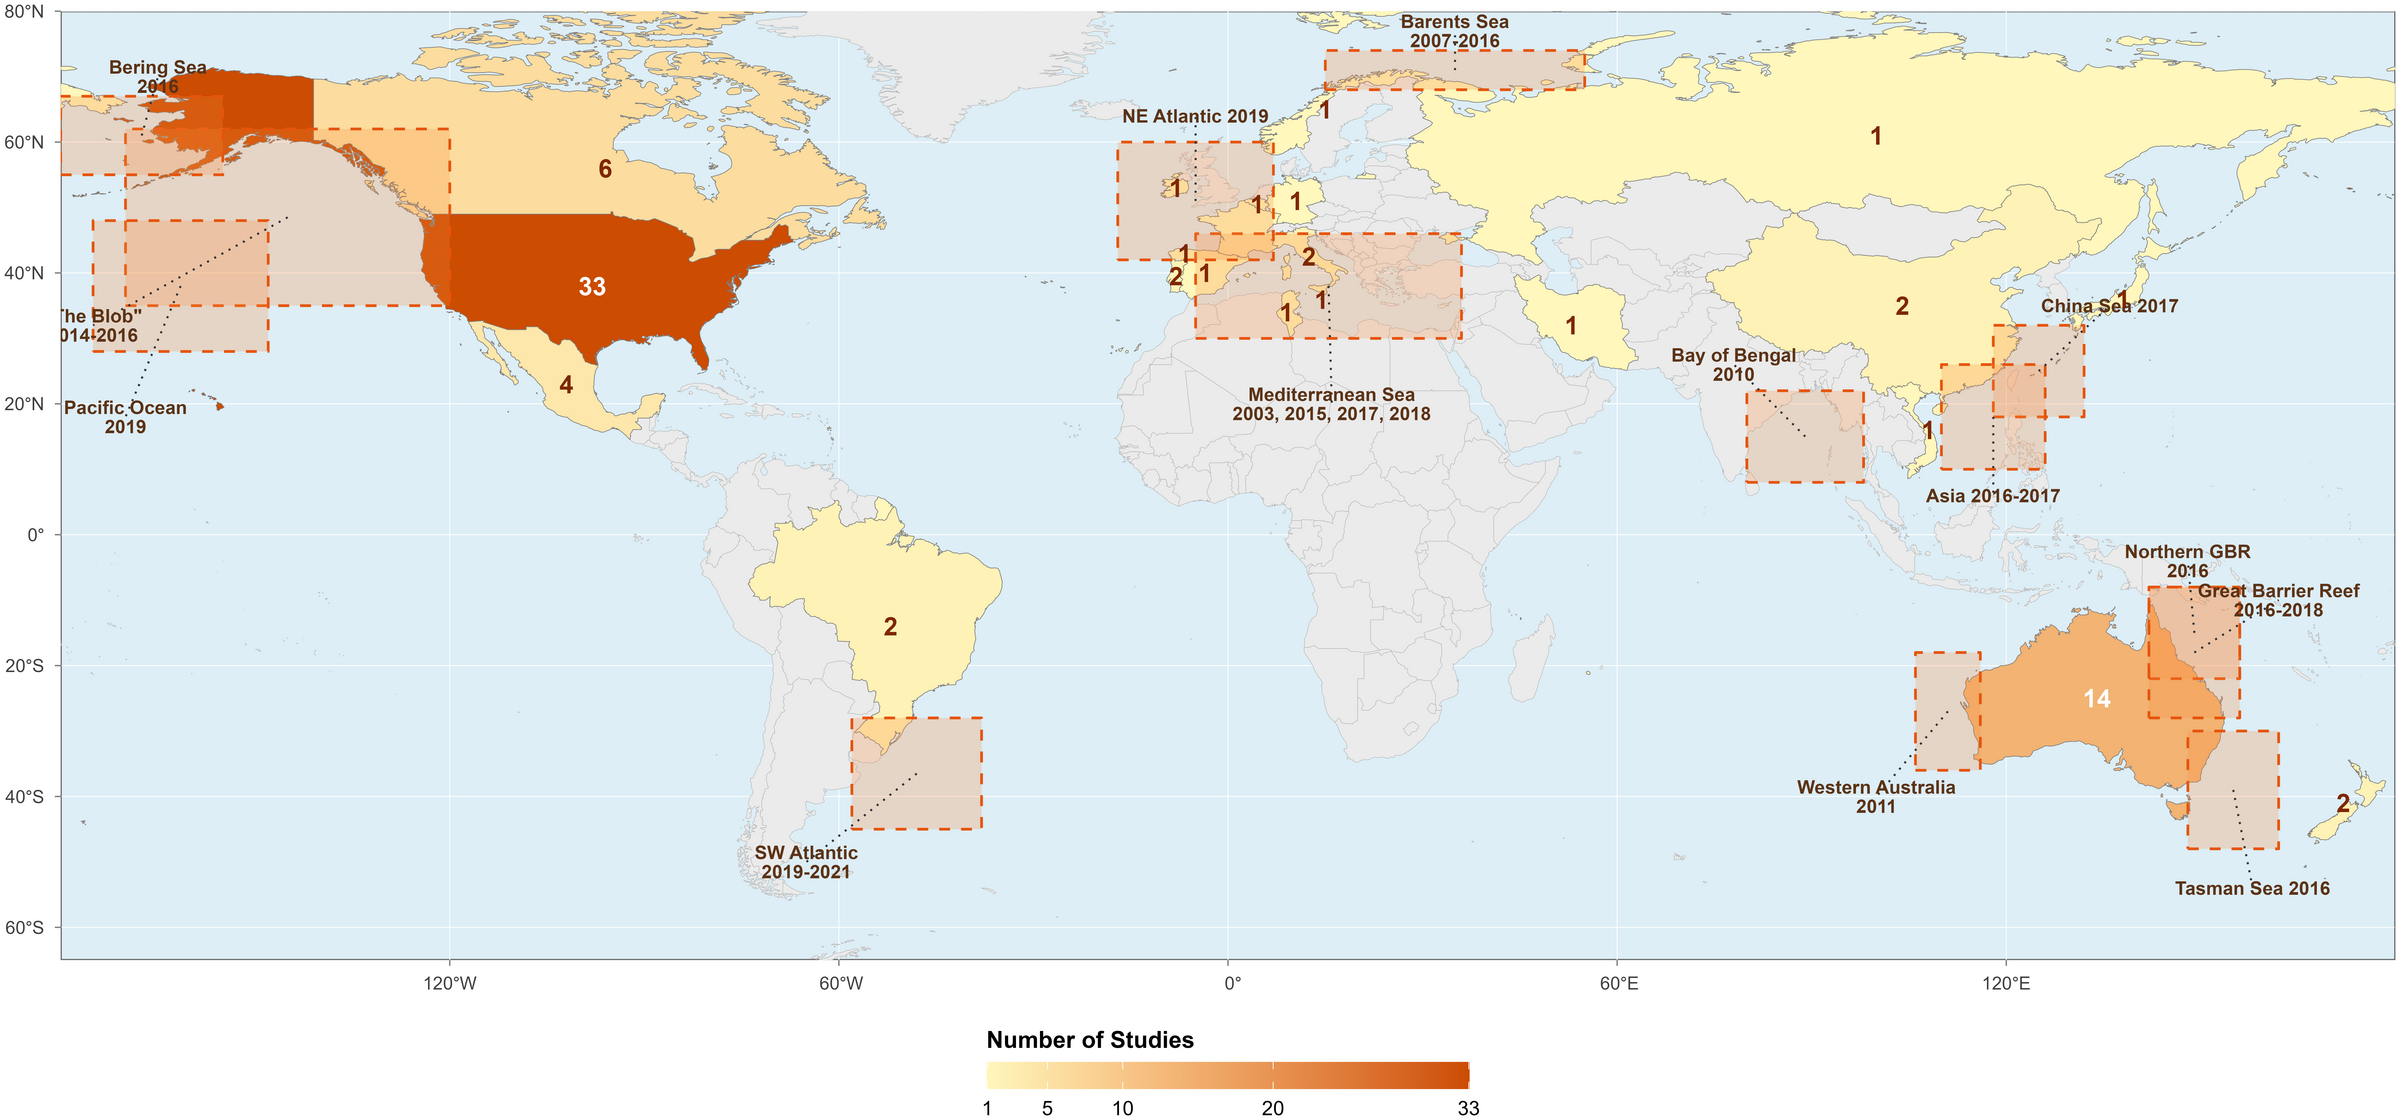
\includegraphics[width=\textwidth]{lit_map}
\caption{Geographic concentration of the evidence base. Country shading and the printed numbers give the number of studies contributed by institutions based in each country; dashed rectangles give the approximate extents of the named marine heatwave events, with their years, to which the studies are linked.}
\label{fig:map}
\end{figure}

\subsection{Modelling frameworks in practice}\label{sec:frameworks}

Table~\ref{tab:frameworks} summarises the framework classes, the inferential question each answers, the dependence structure each represents, the data each requires and the R implementations used in the simulation. The classification is by inferential logic: a GAM used to map habitat suitability is a correlative prediction model, while the same GAM used to estimate a lagged exposure effect is an association model.

\begin{table}[H]
\centering
\caption{Framework classes used to link marine heatwave exposure to biological responses in the 76 reviewed studies. The dependence column states what each class treats as estimable structure; the data column states the minimum data configuration under which the class is identifiable. Software columns name the R implementations used in this review's simulation and widely used alternatives. GLM, generalised linear model; GLMM, generalised linear mixed model; GAM, generalised additive model; DLNM, distributed lag non linear model; GMRF, Gaussian Markov random field; SPDE, stochastic partial differential equation; SDM, species distribution model; BRT, boosted regression trees.}
\label{tab:frameworks}
\small
\setlength{\tabcolsep}{4pt}\begin{tabular}{p{2.5cm}p{3.3cm}p{3.0cm}p{3.2cm}p{2.6cm}}
\toprule
Class & Inferential question & Dependence represented & Minimum data & R implementations \\
\midrule
Association (GLM, GLMM, GAM) & Is exposure related to the response, and how strongly? & None (GLM) or exchangeable random effects for sites or years (GLMM, GAM) & Response and exposure at matched cadence; any sample size the family supports & MASS, lme4, glmmTMB, mgcv \\
\addlinespace
Structured dependence: temporal (AR, state space, DLNM) & When does the response occur relative to exposure, and over how long? & Autocorrelation and lag structure in time & Response series long enough to resolve the lag; at least 3 to 5 cycles of the longest lag & dlnm, MARSS, KFAS \\
\addlinespace
Structured dependence: spatial and spatiotemporal (GMRF\slash SPDE) & How does the effect vary in space, and how much residual spatial structure remains? & Spatially correlated latent field, optionally evolving in time & Observations at enough distinct locations to estimate a range parameter; gridded or irregular & sdmTMB, INLA, VAST \\
\addlinespace
Correlative prediction (SDM, BRT, random forest) & Where will the species be, given covariates? & None explicit; captured implicitly through covariates & Occurrence or abundance with covariate fields; cross-validation blocked in space or time & dismo, ranger, gbm \\
\addlinespace
Experimental and quasi experimental & Does exposure cause the response? & Controlled by design (randomisation, before after control impact) & Replicated treatments or a credible control series & Standard linear and mixed models \\
\addlinespace
Ecosystem and end to end (Ecopath, Ecosim, EcoTroph) & How do impacts propagate through the food web? & Trophic linkages and mass balance & Diet matrices, production and consumption ratios, biomass time series & Rpath \\
\bottomrule
\end{tabular}
\end{table}

\paragraph{Association models dominate by default.}
Generalised linear and mixed models link event metrics to responses using fishery dependent and survey data aggregated to weekly or monthly resolution \citep{brown2021,caputi2016,hart2018,mann2021}. They handle zero inflation, overdispersion and nesting without heavy parameterisation, and they are accessible without specialised training; their prevalence reflects the data and the analysts available rather than a judgement about inferential fit. Generalised additive models are comparatively underused despite their suitability for non linear and seasonal responses \citep{becker2019,fredston2023}. Where they have been applied they revealed structure that parametric specifications miss: smooths over lagged intensity exposed delayed effects \citep{abookire2022,blixt2025}, tensor products captured depth by temperature interactions \citep{becker2019}, and derivative summaries flagged candidate regime shifts \citep{blixt2025}. Diagnostics appropriate to smooth models, such as basis dimension checks and concurvity screening, are rarely reported in parametric studies, so undetected non linearity in GLM based estimates cannot be ruled out. Validation in this class is usually limited to residual checks and information criteria; blocked cross-validation and bootstrap uncertainty appear in a minority \citep{benedetticecchi2024,brown2021,gomes2023}.

\paragraph{Structured dependence models are rare and clustered.}
Models that parameterise temporal or spatial covariance can estimate lagged responses, separate cumulative from pulse exposure and map spatially varying effects. In the subset they appear in fewer than 10\% of studies and almost exclusively in intensively monitored systems. Temporal applications include autoregressive and state space models for humpback whale demography \citep{gabriele2022} and distributed lag structures for euphausiid size \citep{robertson2020}. Spatiotemporal applications fit GMRFs through the SPDE approximation: \citet{evans2023} used INLA to show that euphausiid biomass off Vancouver Island peaked during the 2014 to 2016 event with a Pacific Decadal Oscillation signal invisible in aggregated data; \citet{chasco2022} used VAST, which represents the spatial field as a GMRF in the same way as sdmTMB \citep{thorson2019,anderson2022}, to show that market squid expanded their range only in heatwave years; and \citet{lacheheb2024} used geographically and temporally weighted regression to map where moderate events raised New Zealand catches and extreme events lowered them. The validation practices in these studies, which include rolling origin forecasts and spatial or temporal block cross-validation, are not intrinsic to the model class; they are recommended for any model fitted to autocorrelated data \citep{roberts2017} and are simply more often followed by analysts who have already engaged with dependence. The concentration of these methods in a few author groups indicates that the constraint is expertise and data cadence rather than any lack of relevance.

\paragraph{Correlative prediction models are used for hindsight.}
Species distribution models and machine learning methods appear in MHW studies mainly for retrospective attribution: GAM based SDMs for sardine habitat availability \citep{muhling2025}, boosted regression trees for predator redistribution during four Northeast Pacific events \citep{welch2023}, and GAMs for groundfish and bluefin tuna habitat \citep{rooper2021,mcnicholas2024}. Their use for forward prediction is limited because correlative models calibrated on historical conditions assume distributional equilibrium and carry no representation of thermal limits, movement or life history \citep{welch2023,brodie2021}. Vertical redistribution during heatwaves, documented for mesopelagic fishes in the California Current \citep{iglesias2024}, is one example of a response that horizontal habitat models cannot represent.

\paragraph{Experiments supply mechanism; translation remains the problem.}
Controlled exposures quantify thermal maxima, metabolic scope, growth and survival with internal validity that observational designs cannot match \citep{anastasiadi2021,beaudreau2024,horkan2025,spencejones2025}. They show that early life exposure leaves lasting epigenetic marks, that congeneric clams differ sharply in tolerance, and that prior exposure partially buffers later events. Their authors are candid about limits: food replete, predator free conditions may not generalise \citep{spencejones2025}, and single stressor exposures are snapshots \citep{dinh2021}. The 2015 walleye pollock year class failed through interacting stressors rather than temperature alone \citep{rogers2021}, which illustrates why laboratory thresholds are better treated as mechanistic inputs to population models than as predictors of field outcomes. Quasi experimental designs that exploit natural variation in exposure, such as before after comparisons across the 2014 to 2016 event \citep{horkan2025} and a before after control impact analysis of 227 kelp forest taxa \citep{liang2024}, preserve field realism while supporting causal claims, but remain rare.

\paragraph{Ecosystem models are proofs of concept.}
Mass balance models have shown that trophic structure mediates impact: top down regulated reefs can lose most of their biomass under extreme events while bottom up systems are partly buffered \citep{artana2024}, and recovery time scales with latitude and trophic position \citep{guibourd2024}. Both studies required diet matrices, production ratios and long biomass series that exist only for intensively monitored sites. Hierarchical pooling of parameters across habitat types is the most plausible route to wider application.

\paragraph{Mixed designs.}
Since 2021 a small number of studies have combined approaches, pairing climate projections with controlled experiments \citep{moore2023} or field observation with targeted manipulation \citep{spencejones2025}. Modelling remains the dominant approach every year, experimental studies are fewer but persistent, and mixed designs have appeared only recently (Fig.~\ref{fig:approaches}). Population, distribution and community endpoints are addressed almost entirely by modelling because the relevant scales exceed what can be manipulated; physiological endpoints carry the highest experimental share.

\begin{figure}[H]\centering
\panel{a}{0.49\textwidth}{lit_approach_by_year}\hfill\panel{b}{0.49\textwidth}{lit_approach_by_family}
\caption{Study approaches in the 76 studies. (a) Annual number of publications using experimental, mixed and modelling designs, 2016 to 2025. (b) Number of studies by approach within each response family; a study contributing to several families is counted in each.}
\label{fig:approaches}
\end{figure}

\subsection{Three structural problems}\label{sec:problems}

Three problems recur across the synthesis and motivate the simulation. The measurement foundation is heterogeneous: baseline, threshold and aggregation choices are often unreported and always consequential, so reported effect sizes are not on a common scale. Framework choice follows data infrastructure and training rather than the inferential question, so lagged and non linear responses are systematically under represented in the estimates that enter the literature. And methods are reported at a level of detail that does not support re-implementation, so practice diffuses slowly from the hubs where it is developed. The first problem is a matter of reporting standards. The second is an empirical claim about estimator behaviour, and Section~\ref{sec:simulation} tests it.

% sections/simulation.tex -- design, methods, declaration, then results
\section{A simulation study of modelling frameworks}\label{sec:simulation}

\subsection{Aims and design}\label{sec:simdesign}

The simulation asks a narrow question: when the true biological response to MHW exposure is lagged and mildly non linear, and the data have the site by year panel structure typical of fisheries monitoring, how well do the modelling frameworks found in the literature recover the exposure effect, and how reliable are the uncertainty statements they produce? Aims, data generating mechanism, estimands, methods and performance measures were fixed in advance \citep{morrisgao2021}, and the implementation is deposited in full (Section~\ref{sec:software}). Table~\ref{tab:design} summarises the design.

\begin{table}[H]
\centering
\caption{Factorial design of the simulation. Exposure depends only on region, grid size, spatial range and replicate, so each of the \nPanels{} unique exposure panels is computed once and reused across the nine combinations of effect size and lag.}
\label{tab:design}
\small
\begin{tabular}{p{6.6cm}p{7.2cm}r}
\toprule
Factor & Levels & $n$ \\
\midrule
Region (real OISST series) & Western Australia; Northwest Atlantic; Mediterranean & 3 \\
True effect $\beta_1$ (per $^{\circ}$C day of lagged cumulative intensity) & $-0.04$; $-0.08$; $-0.12$ & 3 \\
True response lag $L$ (years) & 0; 1; 2 & 3 \\
Spatial correlation range of site noise (km) & 0 (independent sites); 50 & 2 \\
Grid size (sites, 25 km spacing) & 9 ($3 \times 3$); 25 ($5 \times 5$) & 2 \\
\midrule
Scenarios & & \nScenarios{} \\
Replicates per scenario & & \nReplicates{} \\
Unique exposure panels & & \nPanels{} \\
Simulated datasets & & \nDatasets{} \\
Model classes & naive GLM; lag-1 GLM; GAM; DLNM; sdmTMB; random forest & 6 \\
Years per dataset (training / held out) & 41 (38 / 3) & \\
\bottomrule
\end{tabular}
\end{table}

\paragraph{Sea surface temperature.}
Rather than simulate temperature, the study uses three real daily NOAA OISST v2.1 series \citep{banzon2016} bundled with the heatwaveR package \citep{schlegel2018}: the Western Australian shelf, the Northwest Atlantic and the Mediterranean, each spanning 1982 to 2022 (14,975 days). Real series carry the seasonality, autocorrelation, warming trend and pulse statistics that make MHW exposure difficult to model, and they are available to anyone with the package installed.

\paragraph{Event detection and exposure.}
MHWs were detected with heatwaveR using the \citet{hobday2016} defaults: a 1983 to 2012 climatology, the 90th percentile threshold with a 31 day smoothing window, a five day minimum duration and a two day maximum gap for joining events. Figure~\ref{fig:events} shows the detection on each series around its most intense event. On the Western Australian series the canonical algorithm identifies the 2011 event from 6 February to 6 April (\waDur{} days), with maximum intensity \waMax{}\,$^{\circ}$C above climatology and cumulative intensity \waCum{}\,$^{\circ}$C days; it is the most intense event in the series by peak anomaly, although a longer 1999 event exceeds it on the cumulative metric (the full series with every detected event is shown in Online Resource 1, Fig.~S4). These values are regenerated by a verification script on the analyst's machine and stored as the reference against which the test suite checks, because detection output can shift between package versions. The sensitivity of the 2011 event to three climatology windows and two percentile thresholds is reported in Online Resource 1, Table S5. Annual exposure per site was summarised as cumulative intensity above threshold ($i_{\mathrm{cum}}$, $^{\circ}$C days), maximum and mean positive anomaly, days above threshold, event count and onset day.

\begin{figure}[H]\centering
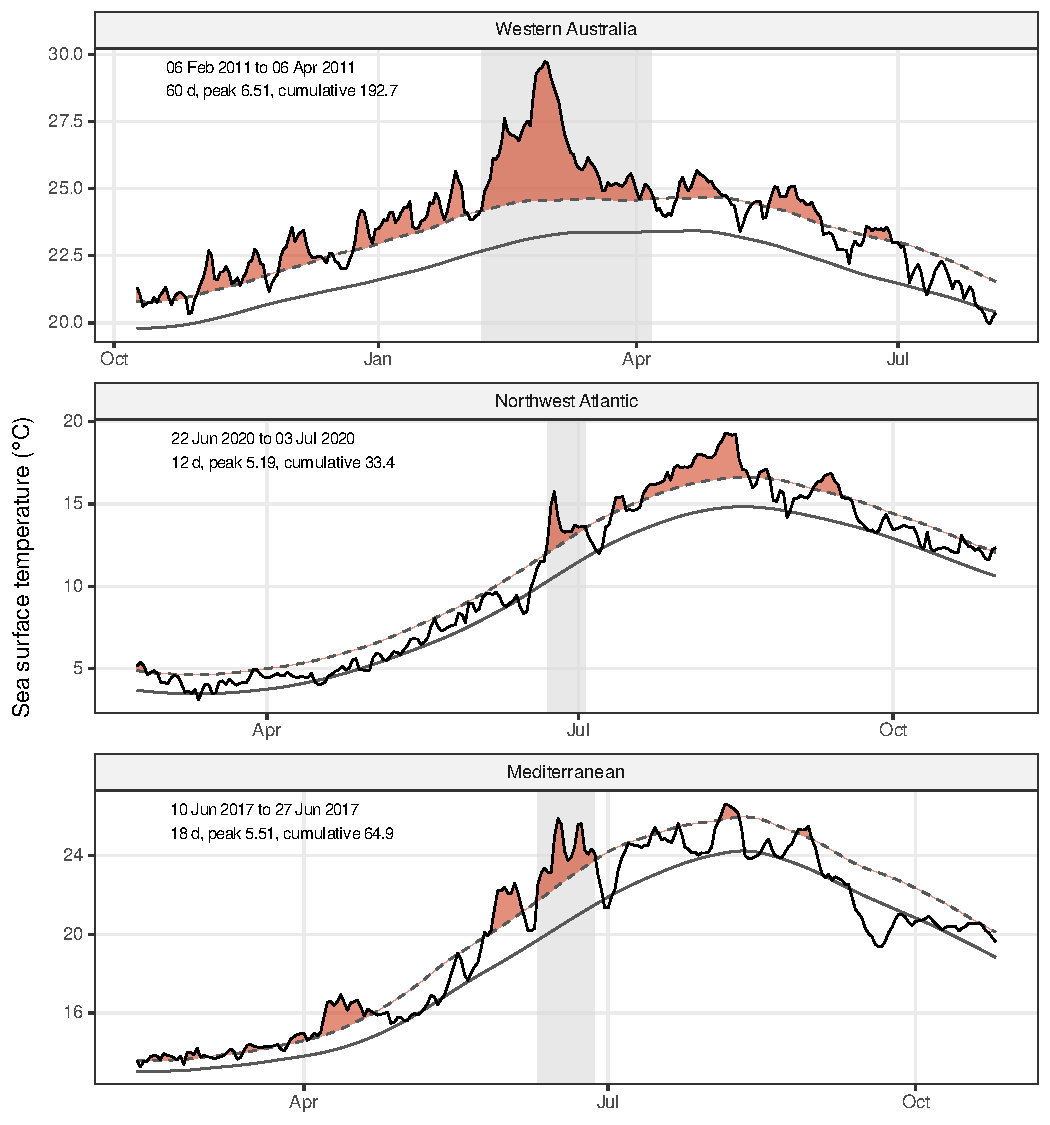
\includegraphics[width=0.92\textwidth]{fig_detection_events}
\caption{Marine heatwave detection on the three real OISST series used in the simulation, each shown for 120 days either side of its most intense event by peak anomaly. Black, daily sea surface temperature; solid grey, seasonal climatology; dashed grey, 90th percentile threshold; shaded, exceedance above threshold; grey band, the detected event with its start, end, duration, peak intensity ($^{\circ}$C) and cumulative intensity ($^{\circ}$C days). Values are as computed by heatwaveR \heatwaveRVersion{} with the Hobday et al. (2016) defaults.}
\label{fig:events}
\end{figure}

\paragraph{Spatial panels.}
Each region's series was replicated across a square grid of sites 25 km apart, with 9 or 25 sites, and a daily noise field with standard deviation 0.3\,$^{\circ}$C was added. The noise was either independent across sites or correlated with an exponential (Mat\'ern $\nu = 1/2$) covariance of range 50 km. Every site therefore shares the real regional trajectory while differing in the timing and magnitude of individual exceedances. Detection and exposure summaries were computed separately for every site.

\paragraph{Data generating process.}
Counts $y_{s,t}$ for site $s$ and year $t$ were drawn from a negative binomial distribution with mean $\mu_{s,t}$ and dispersion $k = 4$, where
\begin{equation}
\log \mu_{s,t} = \alpha + \beta_1 z_{s,t-L} + \beta_2 z_{s,t-L}^{2} + \varepsilon_{s,t}, \qquad \varepsilon_{s,t} = \rho\,\varepsilon_{s,t-1} + \eta_{s,t},
\label{eq:dgp}
\end{equation}
$z$ is $i_{\mathrm{cum}}$ in $^{\circ}$C days, $L$ is the true response lag in years, $\alpha = 2.5$, $\beta_2 = -5 \times 10^{-4}$, $\rho = 0.4$ and the innovations $\eta$ give $\varepsilon$ a stationary standard deviation of 0.3. The quadratic term is small relative to $\beta_1$ but not zero; it represents the saturating behaviour that thermal performance curves imply \citep{sinclair2016} and that linear specifications cannot absorb. With $\alpha = 2.5$ and the observed exposure distributions, mean counts fell between 3 and 7 and the proportion of zeros between 26\% and 44\% across all design cells (Online Resource 1, Table S6), so no cell produced a degenerate response. The response contains no latent spatial field of its own: the only spatial structure is the correlation among site exposure series, which matters for how the spatial model's results are read (Section~\ref{sec:sdmtmb}).

\paragraph{Why lags of zero, one and two years.}
The lag levels follow from the annual cadence of the response and from the response timings documented in the reviewed studies. A lag of zero represents responses that unfold within the year of the event, such as mortality and displacement of adults during the 2011 Western Australian event \citep{caputi2016,yang2019}. A lag of one year represents settlement and recruitment mediated responses, in which the cohort spawned during the event determines the following year's index: the near failure of the 2015 walleye pollock year class \citep{rogers2021} and post settlement cod abundance in the Gulf of Alaska \citep{abookire2022,almeida2024} are of this kind. A lag of two years represents impacts that reach the fished or surveyed age classes only after propagating through recruitment, as in the multi year regulation dynamics of Roe's abalone after 2011 \citep{hart2018}. Longer lags are plausible for long lived species, but with 38 training years and a distributed lag cross basis that already spans lags 0 to 3, lags beyond two cannot be separated from the autocorrelation of exposure itself with any precision. The lag set is a single vector in the configuration file and can be extended by readers whose species warrant it.

\subsection{Models and performance measures}\label{sec:simmodels}

Six model classes were fitted to every dataset (Table~\ref{tab:models}); all were fitted to the first 38 years of each panel with the final three years held out. Table~\ref{tab:models} also gives the estimand each class reports for $\beta_1$. The GLMs and sdmTMB report the coefficient directly. For the GAM it was obtained as the ordinary least squares slope of the fitted smooth over the central 90\% of the exposure range; for the DLNM, as the cumulative log rate ratio at an exposure of 10\,$^{\circ}$C days divided by 10; for the random forest, as the change in mean log prediction when lagged exposure is increased by one unit. These are commensurate only when the response is linear, and their divergence under curvature is part of what the study measures.

\begin{table}[H]
\centering
\caption{Model classes fitted in the simulation, the R implementation used, and the quantity each reports as the estimate of $\beta_1$. NB, negative binomial; GLM, generalised linear model; GAM, generalised additive model; DLNM, distributed lag non linear model; SPDE, stochastic partial differential equation; AR1, first order autoregressive.}
\label{tab:models}
\small
\begin{tabular}{p{2.4cm}p{5.6cm}p{2.4cm}p{3.6cm}}
\toprule
Class & Specification & Package & Estimate of $\beta_1$ \\
\midrule
Naive NB GLM & $y \sim i_{\mathrm{cum},t}$ + site fixed effects; the dominant approach in the reviewed literature & MASS \citep{venables2002} & Coefficient on contemporaneous exposure \\
Lag-1 NB GLM & $y \sim i_{\mathrm{cum},t-1}$ + site fixed effects & MASS & Coefficient on one year lagged exposure \\
NB GAM & $y \sim s(i_{\mathrm{cum},t-1}, k = 6)$ + site random effect, REML & mgcv \citep{wood2017} & OLS slope of the fitted smooth over the central 90\% of exposure \\
DLNM & Cross basis over lags 0 to 3 (natural splines; 3 df exposure, 2 df lag) + site fixed effects, quasi Poisson & dlnm \citep{gasparrini2011} & Cumulative log rate ratio at exposure 10 divided by 10 \\
sdmTMB & $y \sim i_{\mathrm{cum},t-1}$ + Mat\'ern SPDE spatial field + AR1 spatiotemporal field, NB2, 25 km mesh cutoff & sdmTMB \citep{anderson2022,lindgren2011} & Fixed effect coefficient \\
Random forest & $y \sim i_{\mathrm{cum},t}, i_{\mathrm{cum},t-1}$, days above threshold, coordinates; 300 trees & ranger \citep{wright2017} & Finite difference in mean log prediction per unit lagged exposure \\
\bottomrule
\end{tabular}
\end{table}

Performance measures were bias, root mean squared error, empirical coverage of nominal 95\% intervals where an interval is defined, the mean negative binomial log predictive density of the held out years, residual Moran's $I$ of site mean residuals using four nearest neighbours, convergence as judged by each package's own diagnostics (sdmTMB's \texttt{sanity()} function for the spatial model, the iteration limit flags of \texttt{glm.nb} for the GLMs), and wall clock time. Fits that triggered a package warning were retained and recorded as not converged rather than discarded, so that the convergence rates reported are not inflated by silent omission. All summaries were computed across replicates within scenario, then across scenarios.

\subsection{Software, reproducibility and use of generative AI}\label{sec:software}

Every step, from detection through aggregation, figure generation and the tables and numbers in this article, is implemented in R \citep[version \rVersion{};][]{rcore2024} with heatwaveR \heatwaveRVersion{}, dlnm \dlnmVersion{}, mgcv \mgcvVersion{}, sdmTMB \sdmtmbVersion{} and ranger \rangerVersion{}, and released as a tested repository (Data availability). A verification script regenerates the detection reference values on the user's machine and the test suite checks against that file rather than against hard coded numbers. Panel level checkpointing allows the design to be run on a workstation or as a scheduler array job and resumed after interruption; array scripts for SLURM and PBS are included. Every number quoted in Sections~\ref{sec:results} to \ref{sec:discussion} is a macro generated from the deposited output tables.

Generative AI (Claude, Anthropic) was used during preparation of this manuscript for drafting and restructuring code, for drafting prose that was subsequently revised, and for formatting. All code was executed by the author in the environment described above; every numerical result reported here was produced by that execution and reproduced from the deposited outputs before entering the text. The author takes full responsibility for the content.

% sections/results.tex -- every number is a macro from results.tex
\subsection{Results}\label{sec:results}

The five faster model classes were fitted to all \nDatasets{} datasets (\nFitsMain{} fits); the GLMs, GAM, DLNM and random forest returned a point estimate for \glmPctEstimate{}\% of fits, and the small remainder are recorded in the run report (Online Resource 1, Table S12) rather than silently dropped. The sdmTMB model, whose fitting time on spatially independent panels was two orders of magnitude longer than the other classes, was run on \sdmtmbPanelsN{} panels covering \sdmtmbScenarioFrac{} of scenarios (\sdmtmbFits{} fits, \sdmtmbReplicates{} replicates); its results are reported separately in Section~\ref{sec:sdmtmb}. Table~\ref{tab:performance} and Figures~\ref{fig:bias} to \ref{fig:infpred} give the breakdown by model class and lag; Online Resource 1 (Tables S7 to S12) gives every further cut. The text concentrates on the four patterns with consequences for practice.

\performanceTable

\subsubsection{Omitting the lag erases the effect}\label{sec:res-lag}

Figure~\ref{fig:bias} shows the distribution of mean bias in $\hat\beta_1$ across scenarios, by model class and true lag. When the true response was contemporaneous, the naive GLM carried a bias of \naiveBiasLagZero{}, the curvature induced bias that every linear in exposure model conditioning on the correct lag shares (Section~\ref{sec:res-coverage}). When the true lag was one year its bias changed sign and rose to \naiveBiasLagOne{}, and at two years to \naiveBiasLagTwo{}. Against true effects of $-0.04$ to $-0.12$, these biases correspond to under estimation of the effect magnitude by \naiveRelBiasLagOne{}\% at a one year lag and \naiveRelBiasLagTwo{}\% at two years (Fig.~\ref{fig:relbias}). The estimate does not become noisy; it becomes a precise estimate of a much smaller number. In an applied study it would read as a weak or absent effect, with a narrow confidence interval to match.

\begin{figure}[H]\centering
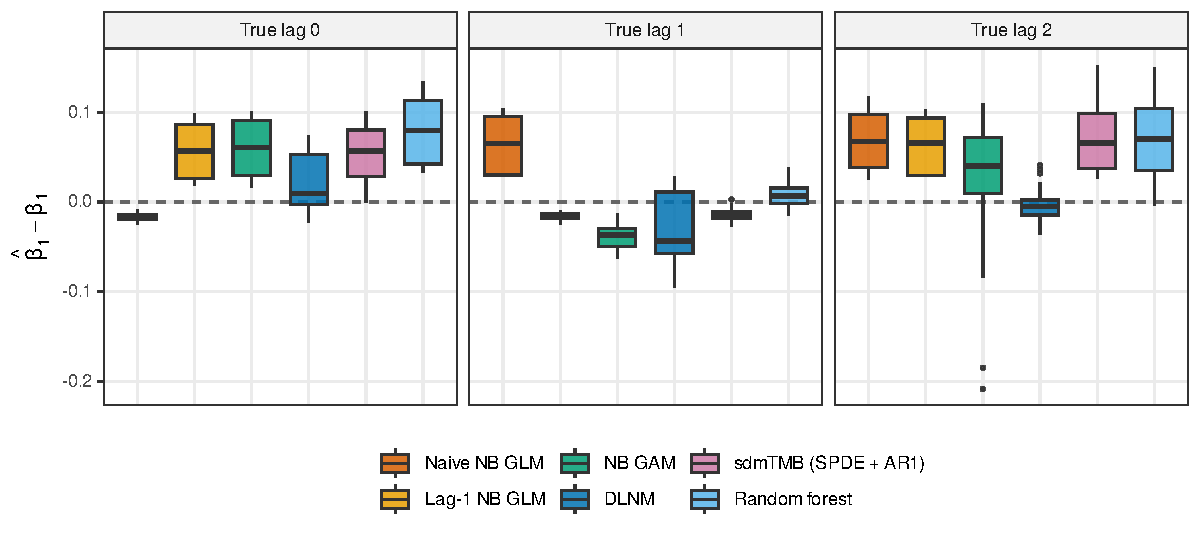
\includegraphics[width=\textwidth]{fig_bias_by_lag}
\caption{Mean bias of the estimated exposure coefficient, $\hat\beta_1 - \beta_1$, across the \nScenarios{} scenarios, by model class and true response lag. Each box summarises one third of the scenarios. The dashed line marks zero bias. Colours identify model classes and are used consistently in all figures.}
\label{fig:bias}
\end{figure}
\begin{figure}[H]\centering
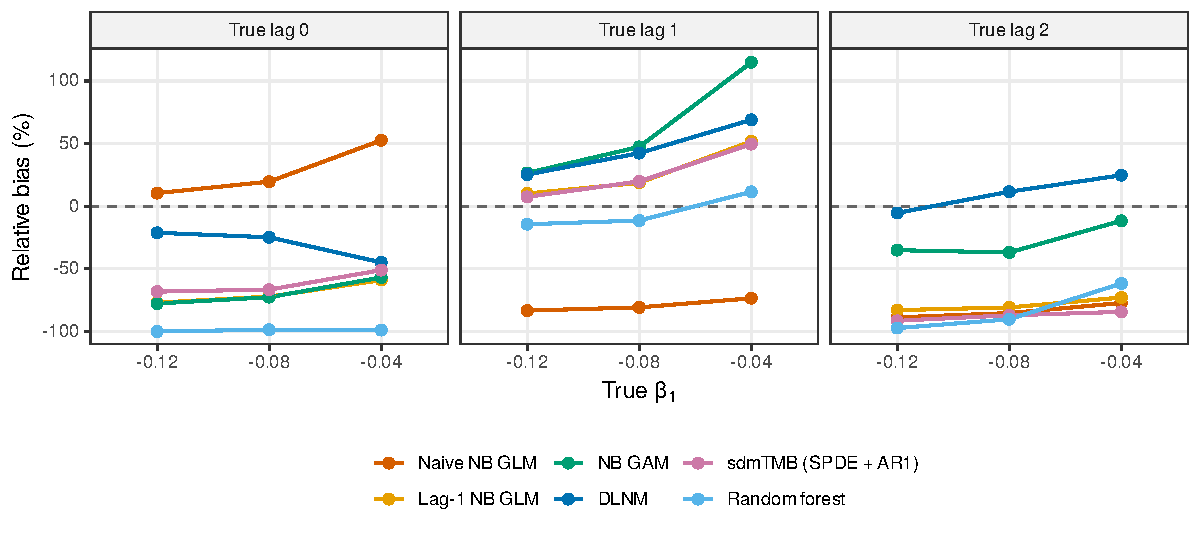
\includegraphics[width=\textwidth]{fig_relative_bias}
\caption{Relative bias, $100(\hat\beta_1-\beta_1)/\beta_1$, by true effect size and true lag. Negative values indicate under estimation of the magnitude of a negative effect.}
\label{fig:relbias}
\end{figure}

The lag aware GLM corrected the problem only when its assumed lag was the true one. At a one year lag its bias was \lagoneBiasLagOne{} (\lagoneRelBiasLagOne{}\% relative), but at zero and two years it collapsed in the same way as the naive model, under estimating by \lagoneRelBiasWrongLag{} respectively. Specifying a lag is therefore not a safeguard unless the lag is known, which in the reviewed literature it rarely was. The GAM, which also conditions on one year lagged exposure, showed the same dependence on the assumed lag.

The distributed lag model behaved differently. Because it estimates the lag profile rather than assuming it, its bias did not switch sign or magnitude with the true lag: \dlnmBiasLagZero{}, \dlnmBiasLagOne{} and \dlnmBiasLagTwo{} at lags of zero, one and two years, with relative bias between \dlnmRelBiasLagZero{}\% and \dlnmRelBiasLagOne{}\%. That robustness came at a cost in precision. The across replicate standard deviation of its estimate at a one year lag was \dlnmSdLagOne{}, against \lagoneSdLagOne{} for the correctly lagged GLM, and its RMSE at that lag (\dlnmRmseLagOne{}) exceeded the correctly lagged GLM's (\lagoneRmseLagOne{}). The practical trade is between an estimator that is accurate only if an unverifiable assumption holds and one that is less precise but does not fail when the assumption is wrong.

\subsubsection{Linear models produce confident intervals around the wrong value}\label{sec:res-coverage}

Nominal 95\% intervals from the two linear GLMs covered the true coefficient in \linearCoverageRange{} of scenarios (Fig.~\ref{fig:coverage}). The failure was not confined to the misspecified lag. Even at the correct lag, where the lag aware GLM's bias was only \lagoneBiasLagOne{}, its coverage was \lagoneCoverageCorrectLag{}, because the small bias induced by the unmodelled quadratic term is large relative to a standard error computed from several hundred site years. The intervals are correctly computed for the fitted model; they are centred on an estimate that the model cannot move to the right place. The GAM, which can represent the curvature, reached \gamCoverageLagOne{} coverage at the correct lag but fell to \gamCoverageMin{} when the lag was wrong. The DLNM's coverage ranged from \dlnmCoverageMin{} to \dlnmCoverageMax{} across lags (mean \dlnmCoverage{}), below nominal but an order of magnitude above the linear models. No class achieved nominal coverage in every condition, which argues for reporting the coverage behaviour of the chosen model under simulated conditions resembling the study rather than assuming it.

\begin{figure}[H]\centering
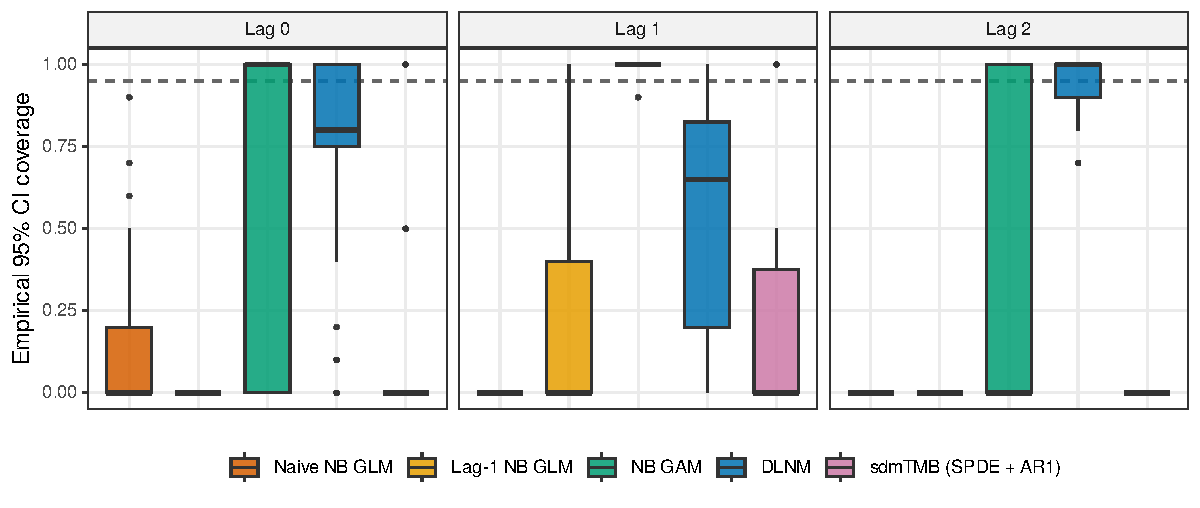
\includegraphics[width=\textwidth]{fig_coverage}
\caption{Empirical coverage of nominal 95\% confidence intervals for $\beta_1$, by model class and true lag. The dashed line marks nominal coverage. The random forest returns no interval and is omitted.}
\label{fig:coverage}
\end{figure}

\subsubsection{The best estimator is not the best predictor}\label{sec:res-prediction}

Held out predictive performance ordered the models differently from coefficient recovery (Fig.~\ref{fig:infpred}). Averaged across all scenarios the naive GLM, with the worst coefficient recovery at non zero lags, produced the highest held out log score (\naiveLogScore{}), followed by the random forest (\rfLogScore{}), the lag aware GLM (\lagoneLogScore{}) and the GAM (\gamLogScore{}). The ordering is driven by the contemporaneous scenarios, where the naive model is correctly specified and predicts well (\naiveLsLagZero{} against \lagoneLsLagZero{} for the lag aware GLM); at a one year lag the lag aware GLM and the GAM predicted better (\lagoneLsLagOne{} and \gamLsLagOne{} against \naiveLsLagOne{}). The random forest, which returns no interpretable coefficient, predicted competitively at every lag and its finite difference effect at a one year lag was nearly unbiased (\rfBiasLagOne{}), although without an interval. The quasi Poisson DLNM has no proper predictive density and was excluded from this comparison. A study that reports a single model cannot show both properties, and the model that would be chosen for prediction is not the one that would be chosen for attribution.

\begin{figure}[H]\centering
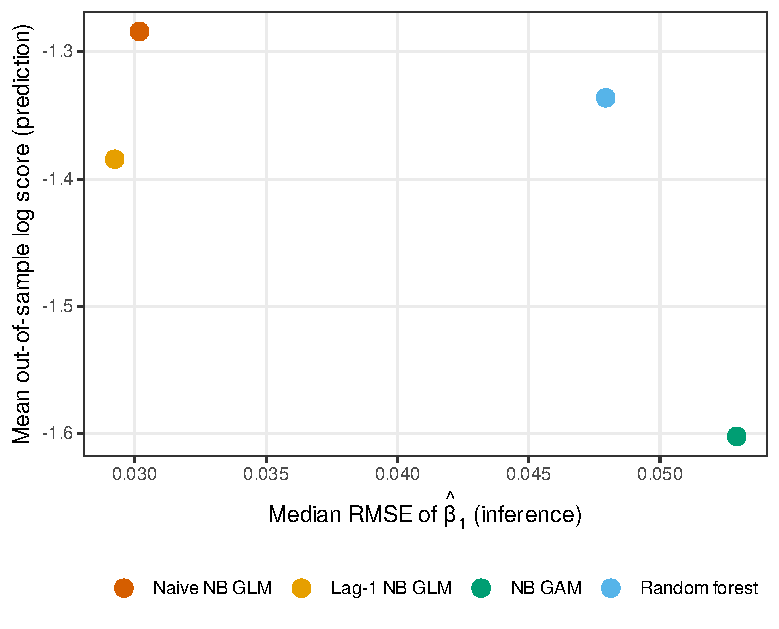
\includegraphics[width=0.6\textwidth]{fig_inference_prediction}
\caption{Coefficient recovery (median RMSE of $\hat\beta_1$ across scenarios) against held out predictive performance (mean negative binomial log predictive density of the final three years), one point per model class. The distributed lag model has no proper predictive density under the quasi Poisson fit and is omitted.}
\label{fig:infpred}
\end{figure}

\subsubsection{Region, grid size and spatial range do not change the ordering}\label{sec:res-region}

The ranking of model classes by absolute bias at a one year lag was \regionRankInvariant{} across the three regions (Fig.~\ref{fig:region}, Online Resource 1, Table S10). The naive GLM's bias at that lag ranged only from \naiveBiasLagOneRegionRange{} across Western Australia, the Northwest Atlantic and the Mediterranean, despite regional exposure distributions whose means differ by more than a factor of two. Grid size and spatial correlation range had no detectable effect on bias for any class (Online Resource 1, Table S11), which is expected because the fixed effect does not depend on the spatial field and the site fixed effects or random effects absorb the correlated noise. Residual Moran's $I$ of site mean residuals was small and negative for all regression classes (\moransIndep{} on independent panels and \moransCorr{} on correlated panels, averaged over models; Online Resource 1, Fig.~S6), confirming that in this design the spatial structure in exposure does not leave residual spatial dependence that a spatial random field would be needed to absorb. The lag problem is therefore not a regional artefact, and it is not alleviated by more sites.

\begin{figure}[H]\centering
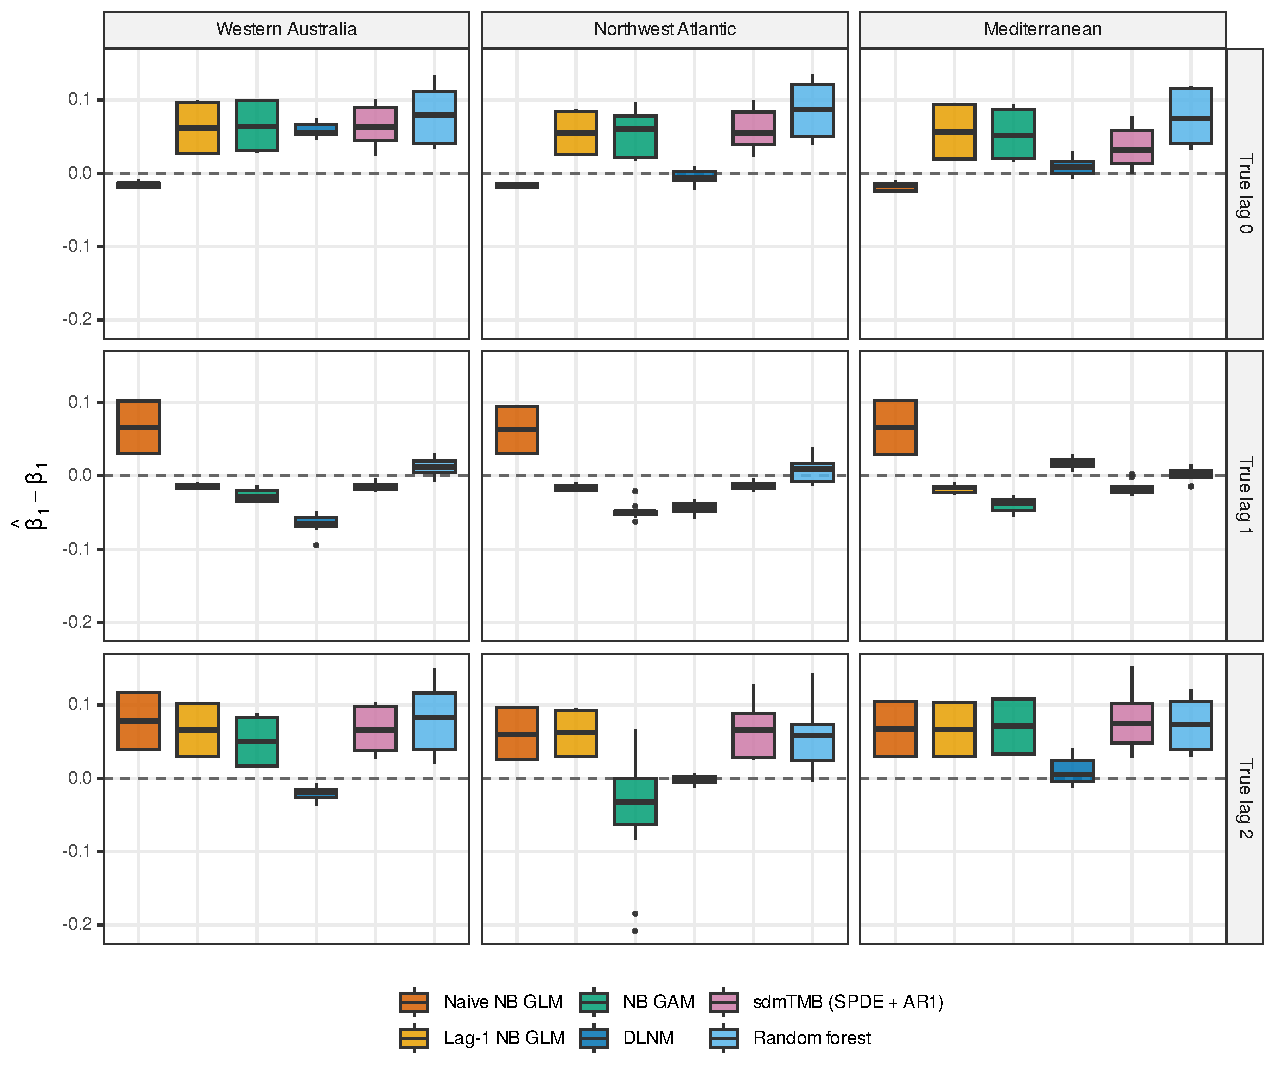
\includegraphics[width=\textwidth]{fig_region}
\caption{Mean bias of the estimated exposure coefficient by region, model class and true lag.}
\label{fig:region}
\end{figure}

\subsubsection{The spatial random field model}\label{sec:sdmtmb}

On the \sdmtmbPanelsN{} panels completed (\sdmtmbFits{} fits), sdmTMB returned point estimates whose bias (\sdmtmbBiasLagZero{}, \sdmtmbBiasLagOne{} and \sdmtmbBiasLagTwo{} at lags of zero, one and two years) tracked the lag aware GLM, as expected for a model that conditions on the same one year lagged covariate. Its \texttt{sanity()} diagnostic flagged \sdmtmbNonConvPct{}\% of fits, most often for a non positive definite Hessian (\sdmtmbNonConvIndep{}\% on spatially independent panels, \sdmtmbNonConvCorr{}\% on correlated ones), and interval coverage was \sdmtmbCoverage{}. These outcomes follow from the design rather than from a defect in the model. Equation~\ref{eq:dgp} contains no latent spatial field in the response; the only spatial structure is correlation among the site exposure series, and the site effects in the fixed effect models absorb it, as the near zero residual Moran's $I$ confirms. sdmTMB is therefore estimating a spatial variance and a spatiotemporal variance that are both truly zero, which places the optimiser at a boundary and is exactly the condition under which the package's documentation warns that the Hessian will be flagged. The design can show that a spatial random field model does not rescue a mis specified lag structure, and that its diagnostics report the absence of a field honestly; it cannot show the conditions under which such a model recovers a spatially varying effect, which would require a different data generating process (Section~\ref{sec:discussion}). Median fitting time was \sdmtmbMedianSec{}\,s per fit, against \naiveSec{}\,s for the GLM, which is the practical reason the model was run on a subset of the design.


% sections/roadmap.tex
\section{A practical roadmap}\label{sec:roadmap}

The synthesis identifies what the literature does; the simulation shows what some of those choices cost. This section turns both into practice. The workflow, the reporting standards and the pitfalls table are implemented in the companion repository, so that each recommendation can be checked against running code rather than taken on trust.

\subsection{A seven step workflow}\label{sec:workflow}

\paragraph{1. State the inferential target before touching data.}
Attribution (did this event change this population?), effect estimation (by how much per unit of exposure?) and forecasting (what happens under the next event?) call for different model classes, different validation schemes and different reporting. Table~\ref{tab:frameworks} maps targets to classes. Declaring the target first prevents the most common failure in the reviewed literature, which is to fit an association model because the data permit it and then interpret its coefficient as if it were a forecast.

\paragraph{2. Detect events from a reproducible temperature source with stated parameters.}
Use a maintained detection implementation and report the data product, its version, the climatology window, the percentile, the minimum duration and the gap rule. Verify the implementation against a documented event before use; this review's verification found that figures circulating for the 2011 Western Australian event did not match the canonical algorithm's output on the same data, which would have propagated into every downstream number had the check been skipped. Report at least one alternative baseline (Online Resource 1, Table S5 gives the template).

\paragraph{3. Compute exposure metrics that span the dimensions the biology may respond to.}
Peak anomaly, mean anomaly, cumulative intensity, days above threshold and onset timing capture severity, integrated dose and phenological alignment respectively. Choosing a single metric for convenience risks discarding the dimension the population responds to; the biological rationale for any narrower choice should be stated in advance.

\paragraph{4. Align exposure to the response cadence without discarding lag structure.}
Where the response is annual, carry exposure for the current and at least two preceding years as separate covariates, and where life stages are known, compute exposure over stage specific windows. The simulation puts a number on the cost of aggregating away the lag.

\paragraph{5. Fit at least one model from each of two classes.}
An inference oriented model that returns an interpretable coefficient with a defensible interval, and a prediction oriented model evaluated on held out data. The simulation shows that these are not the same model, and reporting only one leaves the reader unable to judge the other property.

\paragraph{6. Validate with structure respecting schemes and diagnose residual dependence.}
Hold out contiguous years or contiguous sites rather than random observations \citep{roberts2017}, and report residual temporal and spatial autocorrelation. A significant residual Moran's $I$ from an association model is a direct signal that a structured dependence model should be considered.

\paragraph{7. Deposit code, exposure layers and session information.}
Derived exposure layers are the expensive and irreproducible part of most analyses; depositing them with the detection parameters allows others to reuse the exposure while fitting alternative response models.

\subsection{Minimum reporting standards}\label{sec:reporting}

Table~\ref{tab:reporting} lists nine items that a reviewer can check. They are framed as disclosures rather than prescriptions: a study may defensibly use a 10 year baseline or a single exposure metric, but it should say so and say why. Items 5 and 6 are elevated by the simulation evidence: unreported lag handling and untested curvature are the two choices with the largest measured consequences for the estimated effect.

\begin{table}[H]
\centering
\caption{Minimum reporting standards for MHW impact studies. Items 5 and 6 are rated critical on the basis of the simulation in Section~\ref{sec:results}.}
\label{tab:reporting}
\small
\begin{tabular}{clp{9.2cm}}
\toprule
 & Item & What to report \\
\midrule
1 & Exposure source & Product, version, native resolution, any regridding, and whether the climatology is the provider's or the analyst's \\
2 & Baseline & Window, fixed or shifting, and at least one sensitivity baseline \\
3 & Event definition & Percentile, minimum duration, gap rule, smoothing window; implementation and version \\
4 & Exposure metrics & Which of peak, mean, cumulative, duration and onset were used, and the biological rationale for the choice \\
5 & Lag structure (critical) & Whether a lag was assumed, tested or estimated; lags probed; full lag profile if a distributed lag model was used \\
6 & Curvature (critical) & Whether non linearity was tested; the basis and its dimension if a smooth was used \\
7 & Validation & Scheme (temporal block, spatial block, rolling origin); held out metric; residual autocorrelation test \\
8 & Model classes & At least one inference oriented and one prediction oriented model, with the estimand of each stated \\
9 & Code and data & Repository, session information, deposited exposure layers \\
\bottomrule
\end{tabular}
\end{table}

\subsection{Pitfalls and remedies}\label{sec:pitfalls}

Table~\ref{tab:pitfalls} collects the recurring errors in the reviewed literature together with the remedy that the workflow supplies. Severity ratings for the first two rows are quantitative, taken from the simulation; the remainder are qualitative judgements grounded in the synthesis.

\begin{table}[H]
\centering
\caption{Recurring pitfalls, their consequence, and the remedy supplied by the workflow. Severity: critical, where the simulation measured a consequence large enough to reverse a study's conclusion; high, where the synthesis found the practice common and the consequence well established; moderate otherwise.}
\label{tab:pitfalls}
\small
\begin{tabular}{p{3.4cm}p{1.6cm}p{4.6cm}p{4.6cm}}
\toprule
Pitfall & Severity & Consequence & Remedy \\
\midrule
Contemporaneous exposure when the response is lagged & Critical & Effect magnitude under estimated by \naiveRelBiasLagOne{}\% at a one year lag in the simulation; apparent null results & Carry lagged exposure covariates; fit a distributed lag model where the series permits (steps 4 and 5) \\
\addlinespace
Linear exposure term when the response saturates & Critical & Systematic bias of fixed sign and nominal intervals that cover the truth in \linearCoverageRange{} of scenarios & Test a smooth or quadratic term; report the test (step 6) \\
\addlinespace
Unreported or inherited baseline & High & Effect sizes not comparable across studies; the same event yields different intensities under different windows & Report the window and a sensitivity baseline (step 2) \\
\addlinespace
Single exposure metric chosen for convenience & High & The dimension the biology responds to may be the one discarded & Compute the full metric set; justify any subset (step 3) \\
\addlinespace
Random cross-validation on autocorrelated data & High & Inflated apparent skill; over confident forecasts & Block in time or space; report residual autocorrelation (step 6) \\
\addlinespace
A single model class reported & High & Coefficient quality and forecast quality cannot both be judged & Fit one model from each class (step 5) \\
\addlinespace
Laboratory thresholds used as field predictors & Moderate & Interacting stressors and behaviour alter field outcomes & Treat thresholds as mechanistic inputs or priors, not forecasts \\
\addlinespace
Methods described in prose only & Moderate & Results cannot be re-implemented; practice does not diffuse & Deposit code and exposure layers (step 7) \\
\bottomrule
\end{tabular}
\end{table}

\subsection{What is missing}\label{sec:gaps}

Five gaps limit what any workflow can deliver. Sub annual biological data are the first: the cadence mismatch between daily temperature and annual or seasonal biology is what makes lag estimation hard, and standardised monthly larval surveys, weekly environmental DNA series \citep{gold2024} and telemetry would close it more cheaply than any new method. Grid aligned response products are the second: fishery and survey data at management zone resolution cannot be combined with spatial random field models without an explicit downscaling step, and agencies that publish grid aligned products remove that barrier. Cold anomaly and compound event metrics are the third: fewer than 1\% of studies considered cold events, and the simulation's coverage result applies with greater force where multiple stressors are modelled as one. Intermediate complexity models that embed a single mechanistic constraint, such as a laboratory derived thermal performance curve, inside a correlative framework are the fourth; the components exist in current software but worked examples are rare. Empirical datasets from tropical and Global South regions are the fifth, and the cross regional consistency of the simulation results indicates that this gap is one of data rather than of method.

% sections/discussion.tex
\section{Discussion}\label{sec:discussion}

\subsection{What the simulation adds to the synthesis}

The review found that association models fitted to contemporaneous, linearly specified exposure dominate the literature. The simulation establishes what that habit costs under conditions that resemble the reviewed data: annual site by year panels, counts with overdispersion, and a true response that is delayed and mildly saturating. The naive GLM did not merely lose precision; it returned estimates close to zero when the true lag was one year or more, which in an applied study would read as no detectable effect. A lag aware GLM recovered the effect when the lag it assumed was correct and failed when it was not, which is the practical problem, because the lag is seldom known in advance. The distributed lag model, which estimates the lag profile rather than assuming it, was the only class whose point estimates did not collapse under any lag condition; it paid for that robustness in precision, and its intervals, while covering the truth an order of magnitude more often than the linear models', still fell short of nominal. This ordering does not depend on region, grid size or spatial range, which is the simulation's answer to the question of whether its findings transfer: the mechanism is the mismatch between the model's temporal assumption and the biology's, and that mismatch is indifferent to where the temperature series came from.

The interval results deserve emphasis because they are the least intuitive. Linear models returned standard errors that were correctly computed for the model fitted; their intervals failed because the point estimate was biased by curvature the model could not represent, not because the uncertainty was understated. A reader who sees a narrow, well behaved confidence interval from a GLM has no way to tell, from the interval alone, that it is centred on the wrong value. Only a model that can represent the curvature, or a diagnostic that detects it, reveals the problem. This is why item 6 of the reporting standards is rated critical, and why the workflow asks for a smooth term to be tested even when a linear term is ultimately reported.

The inference versus prediction result is a reminder that model selection criteria encode a purpose. Averaged across the design, the model that predicted held out years best was the naive GLM, whose coefficient was the least trustworthy at non zero lags, and the random forest, which returns no coefficient at all, predicted competitively throughout. Fisheries applications typically need both properties, for attribution and for management advice respectively, and the simulation shows that no single model delivers both. Reporting one model of each class is a cheap safeguard.

\subsection{Scope and limitations of the simulation}

The simulation is a statement about model behaviour under its design, and the design was chosen to be transparent rather than comprehensive. Three limitations bound its reach. The data generating process is a single functional form with one source of non linearity and no interaction between exposure and site; real responses may saturate differently, respond to peak rather than cumulative intensity, or vary with life stage. The panel structure fixes an annual response cadence; studies with seasonal or monthly responses face a different and generally easier lag estimation problem. And the spatial structure enters only through correlated noise in the exposure field, not through spatially varying effects, so the simulation can show whether a spatial random field model recovers a fixed effect reliably but cannot show the conditions under which spatial variation in the effect itself becomes estimable. Each of these is a design choice recorded in a single configuration file, and the repository exists so that readers who find the choices unrepresentative of their system can change them.

The sdmTMB results carry an additional qualification. The model was fitted on \sdmtmbPanelsN{} of the \nPanels{} exposure panels (\sdmtmbScenarioFrac{} of scenarios), because its fitting time was two orders of magnitude greater than the other classes; the subset was selected by replicate order across the design rather than by outcome, so it spans every region, grid size and spatial range. Its diagnostics flagged \sdmtmbNonConvPct{}\% of fits. That figure is a property of the design: the response contains no latent spatial field for the model to estimate, so its variance components sit at zero and the package reports the boundary, as it should. The point estimates nonetheless matched the lag aware GLM's, which is the substantive result: a spatial random field is not a substitute for a lag structure, and the two address different problems. Evaluating sdmTMB where it is intended to excel, with a spatially varying effect or residual spatial dependence in the response, requires a different generating process and is the most useful extension of the repository.

\subsection{Implications for attribution and management}

Retrospective attribution remains the strongest inference that current MHW impact models support, and the reviewed literature contains defensible examples: abalone mortality in Western Australia \citep{caputi2016,hart2018}, squid range expansion in the California Current \citep{chasco2022}, pollock recruitment failure in the Gulf of Alaska \citep{rogers2021}. The simulation does not undermine those studies; it identifies the conditions under which similar studies would understate or miss an effect, and it shows that the fix is inexpensive. Forward prediction is weaker for reasons that are structural rather than methodological: responses are non stationary, lagged and mediated by trophic context, and future events will exceed the thermal range of the training data \citep{frolicher2018,welch2023}. Within those limits, the consistent biological patterns across the reviewed studies, including heightened sensitivity of early life stages, disproportionate impact of short intense events and recovery times that scale with latitude and trophic position \citep{abookire2022,guibourd2024,muhling2025}, are sufficient to support triggered harvest adjustments, temporal protections and exposure conditioned rebuilding timelines even where quantitative forecasts are not.

The geographic concentration of the evidence base is the gap that neither better methods nor better reporting will close. The methods examined here are implementable anywhere that daily temperature and an annual biological index exist, and the temperature side of that requirement is met globally by satellite products. What is missing in the tropical Pacific, the Indian Ocean and the South Atlantic is the biological series, and the regional capacity to analyse it. South to South collaboration, equitable data sharing and hosted computing environments that remove the installation barrier would do more for MHW impact science in those regions than any methodological advance.

\section{Conclusions}\label{sec:conclusions}

Marine heatwave impact assessment has matured into a field with a recognisable methodological architecture: event based exposure definitions, five families of biological response, and a hierarchy of modelling frameworks from association through structured dependence to ecosystem simulation. That architecture is uneven in practice. Association models fitted to contemporaneous, linear exposure dominate because the data and the training permit them, and this review's simulation shows that under lagged and saturating responses they understate effects, miss them entirely, and return confidence intervals that are precise about the wrong value. Distributed lag models correct both problems at modest cost; spatial random field models address a different problem and should be chosen for that reason. No single model served inference and prediction equally. The workflow, reporting standards and pitfalls table offered here are implemented in open, tested R code so that their adoption is a matter of running them rather than reconstructing them. The remaining limits to the field, sub annual biology, grid aligned response data and regional capacity, are limits of data rather than of method, and they are where investment would now return the most.


\section*{Declarations}
\paragraph{Data availability.} The complete R implementation, raw simulation outputs (one row per model fit), summary tables, figure scripts and the LaTeX source of this article are deposited at \url{https://github.com/EAfrifa-Yamoah/mhw-R-audit} and archived at Zenodo (DOI to be inserted at acceptance). The sea surface temperature series are the example data distributed with the heatwaveR package. The literature extraction table is provided as Online Resource 2.
\paragraph{Funding.} No specific funding was received for this work.
\paragraph{Competing interests.} The author declares no competing interests.

\bibliography{refs}

\end{document}
